\newpage
\thispagestyle{empty}
\addtocontents{toc}{\string\contentsline{section}{\protect\hyperlink{appendixa}{APPENDIX - A}}{} \\}
\begin{center}
    {\bfseries \hypertarget{appendixa}{APPENDIX - A} }
    \vspace{1\baselineskip}
\end{center}

%%% PLACE BELOW YOUR APPENDIX %%%
\subsection*{Raspberry Pi 3 Model B+ Specifications} \addtocontents{toc}{\string\contentsline{subsection}{\protect\hyperlink{appendixa}{Raspberry Pi 3 Model B+ Specifications}}{} \\}

    \noindent \textcolor{red}{Example of figure without caption:}
    \begin{figure}[h]
        \centering
        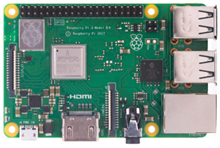
\includegraphics{Images/rpi3-modelB.png}
    \end{figure}



    \noindent \textcolor{red}{Example of table without caption:}
    %%% Use this link for easy way to generate tables with Latex
    %%% https://www.latex-tables.com/
    \begin{table}[h]
\centering
\begin{tblr}{
  width = \linewidth,
  colspec = {Q[148]Q[792]},
  cells = {t},
  hlines,
  vlines,
}
Processor           & {Broadcom
BCM2837B0, Cortex-A53\\64-bit SoC @ 1.4GHz~ ~~}                                                                                                                                                                                                                                                                              \\
GPU                 & Dual
Core VideoCore IV® Multimedia Co-Processor                                                                                                                                                                                                                                                                                        \\
Memory              & 1GB
LPDDR2 SDRAM                                                                                                                                                                                                                                                                                                                       \\
Connectivity        & {\labelitemi\hspace{\dimexpr\labelsep+0.5\tabcolsep}2.4GHz and 5GHz IEEE 802.11.b/g/n/ac wireless LAN, Bluetooth 4.2, BLE (Bluetooth Low Energy)\\\labelitemi\hspace{\dimexpr\labelsep+0.5\tabcolsep}Gigabit Ethernet over USB 2.0 (maximum throughput 300Mbps)\\\labelitemi\hspace{\dimexpr\labelsep+0.5\tabcolsep}4 × USB 2.0 ports} \\
{Video
and \\Sound} & {\labelitemi\hspace{\dimexpr\labelsep+0.5\tabcolsep}1 × full size HDMI\\\labelitemi\hspace{\dimexpr\labelsep+0.5\tabcolsep}MIPI DSI display port\\\labelitemi\hspace{\dimexpr\labelsep+0.5\tabcolsep}MIPI CSI camera port\\\labelitemi\hspace{\dimexpr\labelsep+0.5\tabcolsep}4 pole stereo output and composite video port}           \\
Multimedia          & H.264,
MPEG-4 decode (1080p30); H.264 encode
(1080p30); OpenGL ES 1.1, 2.0 graphics~ ~~                                                                                                                                                                                                                                               \\
SD Card Support     & Micro
SD format for loading operating system and data storage~ ~~                                                                                                                                                                                                                                                                      \\
Input Power         & {\labelitemi\hspace{\dimexpr\labelsep+0.5\tabcolsep}5V/2.5A DC via micro USB connector\\\labelitemi\hspace{\dimexpr\labelsep+0.5\tabcolsep}5V DC via GPIO header\\\labelitemi\hspace{\dimexpr\labelsep+0.5\tabcolsep}Power over Ethernet (PoE)–enabled (requires separate PoE HAT)}                                                    \\
Environment         & Operating
temperature, 0–50°C                                                                                                                                                                                                                                                                                                          \\
Dimensions          & 85 x
56 x 17mm                                                                                                                                                                                                                                                                                                                         
\end{tblr}
\end{table}


\clearpage{}